\section{Simulação e Resultados}\label{sec:experimental}
%

##População inicial, primeiros indviduos gerado##
\begin{figure}[htpb!]
    \centering 
    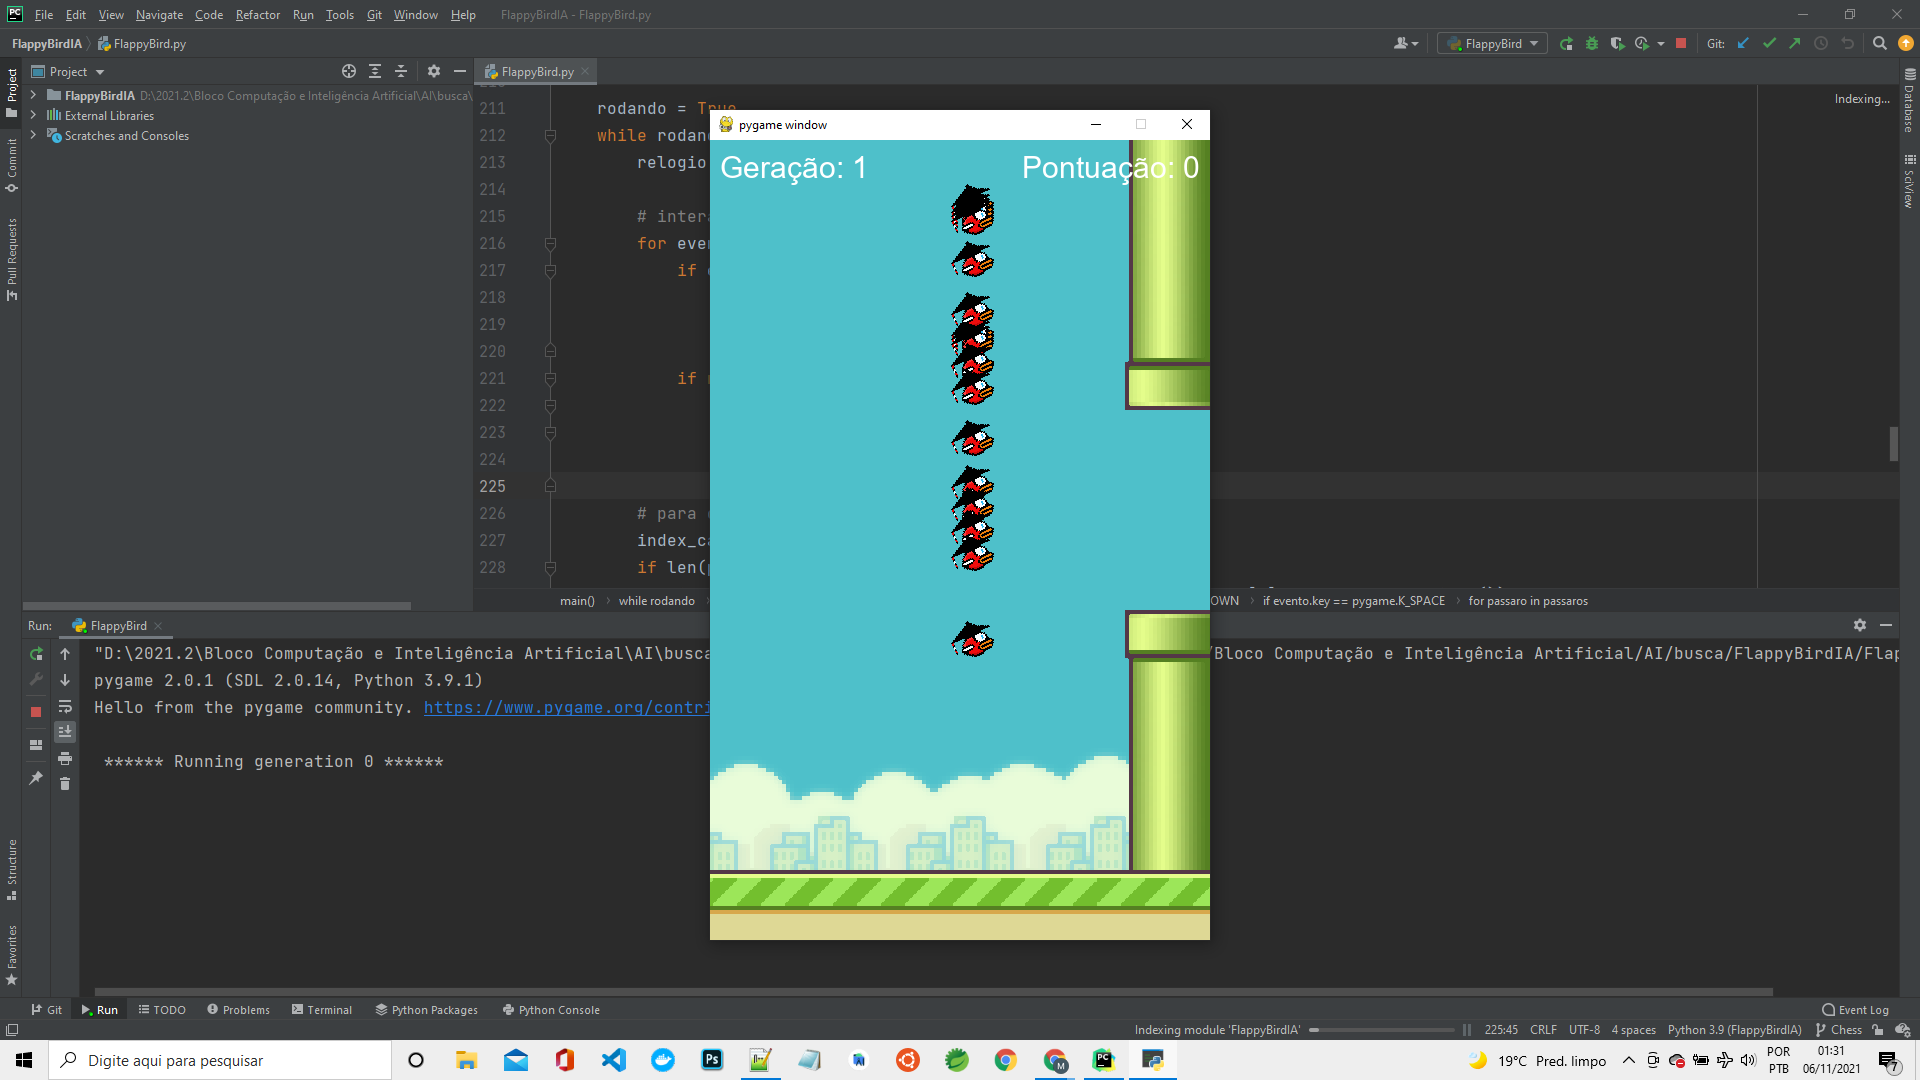
\includegraphics[width=4cm\linewidth]{images/1g_pt0.png}
    
    \caption{Primeira geração.}
    \label{fig:gym}
\end{figure}
\subsection{\textbf{Primeira etapa de teste}}
Nesta etapa de teste foi gerado 100 indivíduos (Redes Neurais)
com 3 entradas e uma saída não tendo camada oculta
a primeira geração a aptidão média da população foi de: 4.56600 
O melhor indivíduo  apto um fitness de: 45,60000 com tamanho: (1, 3)
Primeira espécie de : id 10.
Aptidão média foi ajustada para: 0,050.
A distância genética média é de 1,126, com desvio padrão 0,476.
Uma rede de baixa complexidade um tempo de convergência de 10.764s
O resultado esperado já foi alcançado na segunda geração. 
Com a população de 50 membros em 1 espécie:

\begin{lstlisting}

 ID   age  size  fitness  adj fit  stag
  ====  ===  ====  =======  =======  ====
     1    0    50     45.6    0.050     0

\end{lstlisting}
\begin{figure}[htpb!]
    \centering 
    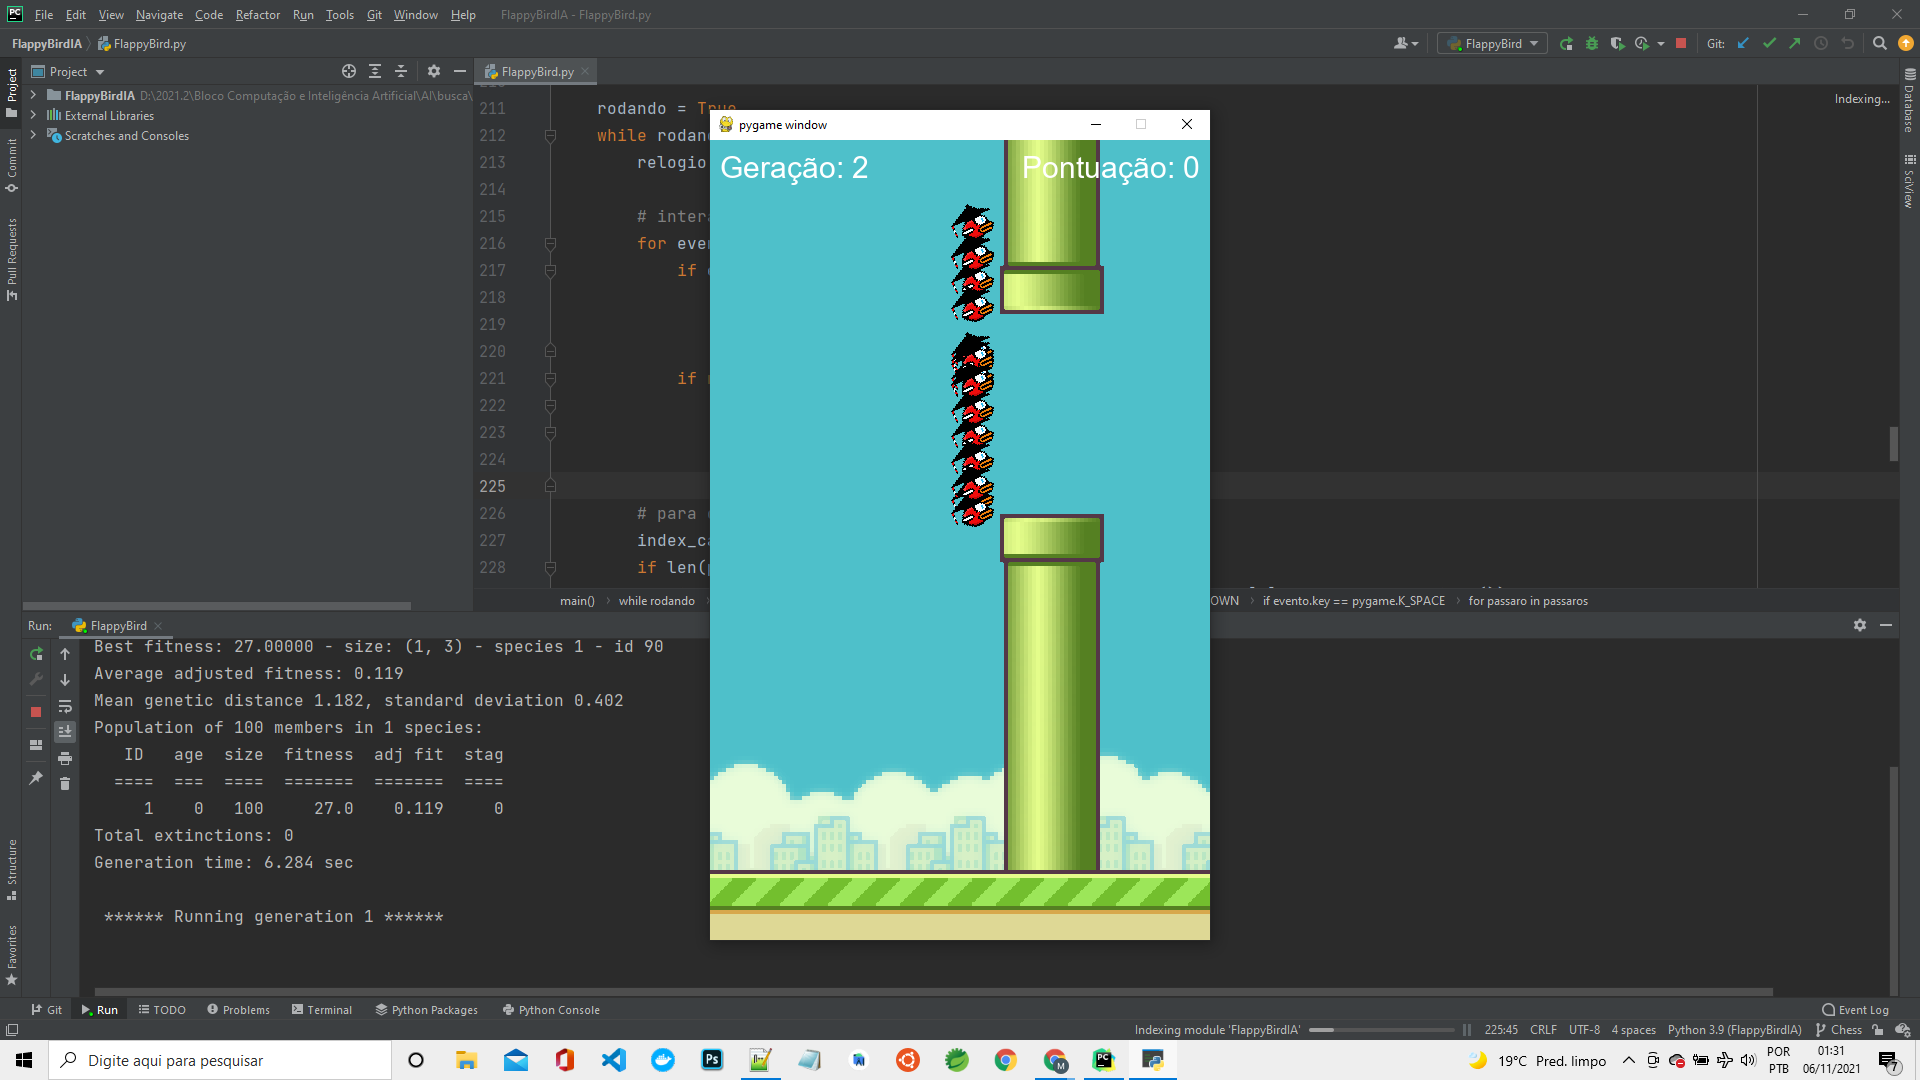
\includegraphics[width=0.6\linewidth]{images/2g_pt2.png}
    \caption{Segunda Geração.}
    \label{fig:gym}
\end{figure}
%

  
\subsection{\textbf{Segunda etapa de teste}}
Nesta etapa de teste foi gerado 100 indivíduos (Redes Neurais)
com 3 entradas e uma saída com 2 camadas ocultas
a primeira geração a aptidão média da população foi de: 4.45400 
O melhor indivíduo  apto um fitness de: 20.10000 com tamanho: (3, 8)
Terceira espécie de : id 3.
Aptidão média foi ajustada para:0.116.
A distância genética média é de 3.251, com desvio padrão 0.504.
Uma rede de uma alta complexidade obteve um tempo de convergência de 5.597 sec na sua primeira Geração.
O resultado esperado não foi alcançado. 
Com a população de 100 membros em 50 espécie:
\begin{lstlisting}

 ID   age  size  fitness  adj fit  stag
  ====  ===  ====  =======  =======  ====
     1    0     2      2.4    0.000     0
     2    0     2      7.6    0.294     0
     3    0     2     20.1    1.000     0
     4    0     2      2.4    0.000     0
     5    0     2      2.5    0.006     0
     6    0     2      2.4    0.000     0
     7    0     2      2.6    0.011     0
     8    0     2      2.4    0.000     0
     9    0     2      2.5    0.006     0
    10    0     2      3.9    0.085     0
    11    0     2      2.4    0.000     0
    12    0     2      2.5    0.006     0
    13    0     2      8.1    0.322     0
    14    0     2      7.5    0.288     0
    15    0     2      3.9    0.085     0
    16    0     2      2.4    0.000     0
    17    0     2      4.0    0.090     0
    18    0     2      2.4    0.000     0
    19    0     2      7.6    0.294     0
    20    0     2      2.4    0.000     0
    21    0     2      3.9    0.085     0
    22    0     2      3.7    0.073     0
    23    0     2      2.4    0.000     0
    24    0     2      2.5    0.006     0
    25    0     2      2.4    0.000     0
    26    0     2      2.6    0.011     0
    27    0     2      7.5    0.288     0
    28    0     2      3.9    0.085     0
    29    0     2      2.4    0.000     0
    30    0     2      2.5    0.006     0
    31    0     2      7.7    0.299     0
    32    0     2      7.5    0.288     0
    33    0     2      7.6    0.294     0
    34    0     2      2.4    0.000     0
    35    0     2      2.5    0.006     0
    36    0     2      2.4    0.000     0
    37    0     2      3.9    0.085     0
    38    0     2      8.0    0.316     0
    39    0     2      3.9    0.085     0
    40    0     2      2.4    0.000     0
    41    0     2      4.0    0.090     0
    42    0     2      7.6    0.294     0
    43    0     2      2.4    0.000     0
    44    0     2      2.5    0.006     0
    45    0     2      3.9    0.085     0
    46    0     2      2.4    0.000     0
    47    0     2      7.5    0.288     0
    48    0     2      7.7    0.299     0
    49    0     2      8.2    0.328     0
    50    0     2      2.4    0.000     0
\end{lstlisting}
\textbf{amostra da geração Nº 36
}
Nesta etapa de teste foi gerado 100 indivíduos (Redes Neurais)
com 3 entradas e uma saída com 2 camadas ocultas
a primeira geração a aptidão média da população foi de: 5.31346 
O melhor indivíduo  apto um fitness de: 46.00000 com tamanho: (3, 7)
Terceira 49 de espécie de: id 147.
Aptidão média foi ajustada para: 0.059.
A distância genética média é de 3.081, com desvio padrão 0.683.
Uma rede de uma alta complexidade obteve um tempo de convergência de 10.759 sec, na sua trigésima sexta geração.
O resultado esperado não foi alcançado. 
A espécie 36 com 2 membros estava estagnada e foi removida
Com a população de 52 membros em 16 espécie:

\begin{lstlisting}
ID   age  size  fitness  adj fit  stag
  ====  ===  ====  =======  =======  ====
     1   36     3      7.6    0.060     5
     2   36     3      7.6    0.048    17
     3   36     3      7.7    0.045    13
     7   36     2      4.1    0.024    17
    14   36     3      7.5    0.047     9
    16   36     2      2.5    0.001     3
    23   36     2      2.6    0.002    12
    25   36     2      3.9    0.017    14
    26   36     3      7.7    0.075    14
    37   36     2      4.0    0.024    18
    38   36     5      8.4    0.124     9
    43   36     3      7.8    0.060     9
    45   36     2      4.0    0.036    16
    48   36     5      7.6    0.088     9
    49   36    10     46.0    0.285     0
    50   36     2      2.7    0.003    14
Total extinctions: 0
Generation time: 10.759 sec (6.202 average)

 ****** Running generation 37 ****** 

Population's average fitness: 15.43077 stdev: 70.67266
Best fitness: 518.50000 - size: (3, 6) - species 49 - id 188

Best individual in generation 37 meets fitness threshold - complexity: (3, 6)
\end{lstlisting}

%
\begin{figure}[htpb!]
    \centering 
    
\includegraphics[width=0.85\linewidth]{images/2g_pt121.png}
    \caption{Os resultados não foram conclusivos.}
    \label{fig:loss}
\end{figure}
%



